\section{Web Information Systems - I Lecture}

\subsection{Introduction and Definition of WIS}\label{introduction-to-web-information-systems}

Good morning! In this class, we will be discussing web information
systems. As usual, you can find the slides on WEBEEP. Let's begin by
defining what a web information system is.

\begin{figure}[!h]
  \centering
  \includegraphics[page=2, trim = 2cm 3cm 2cm 4.5cm, clip, width=\textwidth]{images/03 - Web_Information_Systems.pdf}
\end{figure}

A web information system is a system that facilitates communication
between machines using either the public internet or an IP-based private
VPN. Users can access the system's functionalities through a web
browser. This definition provides a broad understanding of what a web
information system entails.

\paragraph*{Defining Web Information Systems}
The public internet and the IP protocol, along with browsers, have
brought about significant changes in information systems. Any system
that meets two criteria can be considered a web information system.
Firstly, it must be accessible through a browser. Secondly, it should be
connected to the private VPN of the company. This means that even a
traditional ERP with its core functionalities can be classified as a web
information system if it meets these criteria.


\subsection{Impact of Technical Innovations}
These two technical
innovations---internet and browsers (user interfaces)---have resulted in a transformation of the technologies
utilized, even by components of web information systems that were
created prior to the advent of the web. In essence, ERP providers have
reimagined the interface and core technologies of their packages to
align with this new paradigm.

\subsubsection{The Internet and Its
  Influence}\label{the-internet-and-its-influence}

\begin{figure}[!h]
  \centering
  \includegraphics[page=4, trim = 2cm 2.5cm 2cm 1cm, clip, width=\textwidth]{images/03 - Web_Information_Systems.pdf}
\end{figure}

Now, let's discuss the main innovation that revolutionized web
information systems: the internet. The internet connected companies to
individual customers for the first time, marking a significant change in
the business landscape. This not only impacted individual customers but
also the employees working for these companies. The ability to connect
the company's potential market, especially retail customers, through a
public network was seen as a monumental shift.

During the late 90s, when the internet was introduced, there was a great
deal of hope and belief in the transformative power of this new
technology. There was a hype surrounding the web, with expectations that
it would drastically change people's lives in a short period of time.
The paradigm of exponential organization emerged, where companies
without the burden of physical shops or channels to reach customers
could experience rapid growth. As a result, the value of web-based
companies experienced significant growth around the year 2000.

\paragraph{The Dot Com Bubble}\label{the-dot-com-bubble}

The dot com bubble refers to a period when the value of stocks of
companies with websites ending in ``.com'' skyrocketed, far exceeding
their actual revenues and assets. However, this rapid growth was
eventually followed by a significant stock market crash, one of the
largest in recent history. This sudden shift from extreme optimism to
pessimism marked a turning point in the market.

\paragraph{Web Technology in Traditional
  Companies}\label{web-technology-in-traditional-companies}

The web has undoubtedly revolutionized processes for both traditional
and new companies, creating new industries while also causing the
decline of others. However, the pace at which society adapted to these
changes was slower than the expectations of the stock exchange. For
traditional companies to fully benefit from web innovation, they must
first go through the implementation and integration of their information
systems, even with traditional technologies. Without this, it is
challenging for them to compete effectively on the web, unless they have
a history of being highly innovative in their approach to information
systems and are prepared to utilize the web as a new channel to reach
customers.

For instance, companies that lack a unified data system, which is a
fundamental aspect of the ERP paradigm, will struggle to provide a
satisfactory web service. The web is a more objective platform compared
to a physical store, as there is no personal interaction. Customers have
certain expectations for service quality, which are set by industry
leaders. Consequently, the web can actually make the customer
relationship more challenging rather than easier. Only companies that
have successfully integrated previous technologies into their operations
have been able to fully exploit the potential of the web.

\paragraph{Extended ERP and E-Commerce}\label{extended-erp-and-e-commerce}

When examining the functional architecture of ERP systems, it becomes
clear that extended ERP is more influenced by the web than core ERP. The
web has opened up new opportunities, particularly in e-commerce, which
continues to evolve. Extended ERP, which is enabled by the web,
encompasses various functionalities that must be supported by a
well-integrated and IT-supported internal process.

One of the key enabling technologies for extended ERP is CRM, with the
web playing a significant role. While companies have been using
technology, such as Salesforce automation, to interact with customers
for some time, the web has made it easier to showcase services, prices,
and conditions, as well as compare alternative suppliers. This has
created a need for integration across different channels, as any
mistakes or inaccuracies on the web are visible to all. It is no longer
acceptable for customers to have to visit a retail shop for information;
it must be readily available and accurate on the web.

\subsection{E-Commerce and Its
  Evolution}\label{e-commerce-and-its-evolution}

Companies have recognized the importance of integrating customer
information into a single database, commonly known as a customer
database or CRM. This integration, whether referred to as omni-channel
or multi-channel, has become increasingly important as the web has
become the primary access point for both customers and internal users.

\begin{figure}[!h]
  \centering
  \includegraphics[page=5, trim = 2cm 5cm 2cm 4.5cm, clip, width=\textwidth]{images/03 - Web_Information_Systems.pdf}
\end{figure}

Initially, the web was seen as a platform for e-commerce, allowing
companies to sell their products online and reach a wider market. This
was seen as a significant opportunity. E-commerce refers to the buying
and selling of products and services online, primarily targeting retail
customers. On the other hand, when referring to business customers, the
term e-business is used. For example, if a company purchases from
another company online, it is considered e-business. Similarly, if a
public administration buys from a supplier online or provides services
to other public institutions or citizens, it is referred to as
e-government.

In summary, e-commerce focuses on reaching the market and selling
products online, while e-business and e-government encompass a broader
range of online transactions involving business customers and public
administrations, respectively.

\subsection{The Dot Com Trend and Its
  Aftermath}\label{the-dot-com-trend-and-its-aftermath}

In the early days of the dot com trend, many companies initially set up
their e-commerce operations as separate units or even separate
companies. This was a common approach when a new technology brought
about significant changes. These companies lacked the necessary
expertise to effectively manage and leverage the new technology, so they
sought the help of consultants and formed internal teams to handle it.
Over time, these teams evolved into dedicated units focused on the new
technology, such as the web.

\begin{figure}[!h]
  \centering
  \includegraphics[page=6, trim = 1.5cm 4cm 2cm 3cm, clip, width=\textwidth]{images/03 - Web_Information_Systems.pdf}
\end{figure}

This pattern of innovation is not unique to the web; it has been
observed in various industries. However, during the dot com era,
companies that were perceived as pure dot coms, operating solely on the
web without any traditional brick-and-mortar presence, were highly
valued in the stock market. This led even traditional companies to
establish separate units or even separate companies with their own
distinct brands to tap into the potential of the web. For instance, in
2000, Deutsche Bank launched Bank 24, a web-only bank operating as a dot
com.

However, this trend came to a halt after the dot com bubble burst and
the subsequent stock market failure. Even Deutsche Bank eventually
integrated Bank 24 back into its core services, recognizing the need to
reassess their approach in light of the challenges faced by dot com
companies.

\subsection{Integrating Web and Traditional
  Channels}\label{integrating-web-and-traditional-channels}

Companies have recognized the importance of integrating the web as an
additional channel for their existing customers. There are a few reasons
behind this realization. Firstly, companies understood that relying
solely on the web for growth and stock market success was no longer
feasible after the dot com bubble burst. Secondly, they realized that
web-based operations still require physical processes and the management
of people, offices, and complementary services. This led to the
recognition of the synergies between web-based companies and traditional
structures, as Deutsche Bank recognized.

To leverage these synergies, companies brought web-based operations back
into their traditional structures and began integrating the web as a
channel alongside other existing channels. This integration process was
facilitated by customer relationship management (CRM) practices.
Companies started by creating a shared customer database and analyzing
it to understand the evolving habits of web customers. Based on these
insights, they developed innovative services to cater to the changing
needs of web customers over time.

\begin{figure}[!h]
  \centering
  \includegraphics[page=7, trim = 2cm 1.5cm 2cm 1.5cm, clip, width=\textwidth]{images/03 - Web_Information_Systems.pdf}
\end{figure}

Initially, customers were skeptical about making purchases on the web,
especially for high-value or high-quality products. They preferred
traditional brick-and-mortar shops. However, over time, customer
behavior shifted, and e-commerce gained traction across various
industries. The pace of this shift varied across industries, with some
experiencing faster adoption than others. Nevertheless, e-commerce has
become prevalent in almost all industries, including fashion, grocery,
tourism, banking, trading, and learning. Each industry has its own
specific terms and practices related to e-commerce.

\subsection{The Role of E-Commerce
  Post-COVID-19}\label{the-role-of-e-commerce-post-covid-19}

When the internet was first introduced, there were predictions about
which industries would be most impacted by e-commerce and how quickly it
would replace traditional channels. However, it took nearly 20 years for
e-commerce to become pervasive, serving only a small percentage of
transactions and clients. The COVID-19 pandemic changed this
dramatically, giving e-commerce a significant boost. It quickly
developed and penetrated the market, reaching a larger audience. While
there has been a slight decline after the initial surge, e-commerce has
still experienced substantial growth and increased penetration.

\subsection{Customer Journey and Online
  Information}\label{customer-journey-and-online-information}

To illustrate this point, let's consider the example of grocery
shopping. Despite the pandemic, only a small percentage of people
actually do their grocery shopping online. This indicates that the
experience of shopping in a traditional store or through traditional
distribution methods is still considered superior to the online
experience. As a result, the current trend is to view online shopping as
complementary to other channels, rather than a standalone option.

\begin{figure}[!h]
  \centering
  \includegraphics[page=8, trim = 1.5cm 3cm 2cm 3cm, clip, width=\textwidth]{images/03 - Web_Information_Systems.pdf}
\end{figure}

When customers engage with a company, they go through a journey that
involves multiple channels at different stages of the transaction. It
all begins with a need, which may arise from seeing an advertisement or
simply having a requirement. The first step in this journey is typically
going online to gather information. This initial step is crucial in the
transaction process and is usually done through the web. When customers
are unsure of where to make a purchase, they turn to the internet to
find information. This helps them make decisions about the provider, the
brand, and the specific product they want to buy. With the advent of
social media, customers also rely on product reviews to guide their
choices. This search phase of the transaction, where customers seek
information, accounts for approximately 90\% of visits to a company's
website.

\subsection{Designing Effective Web
  Information}\label{designing-effective-web-information}

The main purpose of websites is to provide information to customers who
are looking for products or learning about a company for the first time.
Typically, websites include a general presentation of the company, its
mission, organizational structure, job opportunities, news and events,
and information about its products. Some older websites may offer a
downloadable product catalog in PDF format or a multimedia online
catalog where customers can browse through the products. These websites
often provide recommendations for related products that are commonly
purchased together. Contact information, such as the call center,
company size, and location, is also provided, sometimes with a map for
easy navigation.

When designing the information services of their website, companies are
primarily concerned with providing a positive first impression to
customers who have no prior knowledge of the company. This can be
challenging for companies, as they need to carefully design the
website's navigation structure. It is often best to follow a navigation
structure that is similar to what competitors use, as customers have
certain expectations about where to find specific information on a
company's homepage. Keeping the information provided on the website
standardized is a good idea, although it should be regularly updated as
company information, including the mission, can change over time. To
update the information on their website, companies need to gather the
necessary information from various stakeholders within the organization
who possess the relevant knowledge. This can be a complex task, as
information is often scattered across different departments or
individuals. The website serves as a central access point for customers
to find all the information they need.

\subsection{Quality Criteria for E-Commerce
  Sites}\label{quality-criteria-for-e-commerce-sites}


\begin{figure}[!h]
  \centering
  \includegraphics[page=9, trim = 1.5cm 4.5cm 3cm 4cm, clip, width=\textwidth]{images/03 - Web_Information_Systems.pdf}
\end{figure}

In order to provide consistent information to customers on the web,
information owners must cooperate. There are two approaches to
collecting this information. The first approach is federated, where
there is one central site with a thin layer of information and multiple
local sites where individual business units can provide their own
information. The landing page serves as a collection of links to the
different business units' websites. While this approach allows for
information retrieval to be closer to the business units, it often
results in a website that lacks standardization and has lower overall
quality.

The second approach is to establish an editorial committee that
constantly updates the information on the website. This committee seeks
information from the different business units and follows a common
template for all units, ensuring standardization. Although this approach
is more expensive due to the need for an editorial committee and
agreement on the information to be provided, it generally leads to
higher quality.

\begin{figure}[!h]
  \centering
  \includegraphics[page=10, trim = 2cm 2cm 2cm 4cm, clip, width=\textwidth]{images/03 - Web_Information_Systems.pdf}
\end{figure}

When considering the quality criteria for an e-commerce site, there are
several factors to consider. First, customers expect the content to be
complete, dependable, and correct. They also want consistency in the
information provided by the call center. Second, the structure of the
website should allow customers to easily navigate and understand the
information. A centralized structure is preferable in this regard. The
presentation of the website should have a coherent graphic style to
instill trust and confidence in the company. The layout and position of
information should be intuitive and standardized. Navigation should also
be intuitive, with multiple paths to reach the same information. The
website should be well-connected, allowing customers to navigate between
pages without having to return to the homepage. The ease of navigation,
including the ability to go back multiple steps, is crucial.

In conclusion, the quality criteria for an e-commerce site include
content completeness and dependability, a clear and intuitive structure,
a coherent graphic style, and easy navigation with multiple paths to
reach information.

\section{Web Information Systems - II Lecture}
\subsection{Introduction to Web Information Systems - Part
  Two}\label{introduction-to-web-information-systems---part-two}

Welcome to part two of our series on web information systems. In this
installment, we will delve deeper into the fascinating world of
web-based information systems and explore their various components and
functionalities. So, let's jump right in and continue our exploration of
this exciting topic.

In part one, we introduced the concept of web information systems and
discussed their importance in today's digital age. We learned that web
information systems are designed to collect, process, store, and
disseminate information over the internet. They play a crucial role in
facilitating communication, collaboration, and decision-making in
various domains, such as business, education, healthcare, and
government.

Now, let's move on to the key components of web information systems. At
the heart of any web information system is the web server, which acts as
the central hub for storing and serving web pages and other resources.
The web server receives requests from clients, such as web browsers, and
responds by sending the requested information back to the client.

Another essential component of web information systems is the database.
The database stores and organizes the vast amount of data that is
generated and used by the system. It allows for efficient storage,
retrieval, and manipulation of data, ensuring that the system can handle
large volumes of information effectively.

Web applications are another critical element of web information
systems. These applications are responsible for processing user
requests, generating dynamic content, and providing interactive
features. They enable users to perform various tasks, such as submitting
forms, conducting searches, and accessing personalized information.

To ensure the security and integrity of web information systems,
authentication and authorization mechanisms are implemented.
Authentication verifies the identity of users, while authorization
determines what actions they are allowed to perform within the system.
These mechanisms help protect sensitive information and prevent
unauthorized access.

In addition to these components, web information systems often
incorporate other technologies and tools, such as content management
systems, search engines, and analytics platforms. These tools enhance
the functionality and usability of the system, allowing for efficient
content creation, search capabilities, and data analysis.

In conclusion, web information systems are complex and multifaceted
systems that enable the collection, processing, storage, and
dissemination of information over the internet. They consist of various
components, including web servers, databases, web applications,
authentication and authorization mechanisms, and additional tools and
technologies. Understanding these components is crucial for building and
maintaining robust and effective web information systems. Stay tuned for
part three, where we will explore the design and development process of
web information systems.


\subsection{Gaining Online Visibility}\label{gaining-online-visibility}

Now that we have discussed the quality criteria for websites, let's take
a closer look at what makes a website truly exceptional.

\subsubsection{Search Engines and User
  Behavior}\label{search-engines-and-user-behavior}

Despite having a high-quality website, companies still need to ensure
that their online presence is visible. So, how do companies initiate the
search phase of a transaction? Well, they start by going online and
conducting a search on popular search engines like Google or Bing. It's
worth noting that Google is the most widely used search engine, with a
near monopoly in certain countries, particularly when it comes to web
searches. When conducting a search, people usually look for a specific
product or service.

\subsubsection{Google's Dominance and Search
  Patterns}\label{googles-dominance-and-search-patterns}

In many cases, when you're searching online, you may not know the
specific brand or company name for the product you need. Instead, you
have a general idea of the type of product you're looking for. For
instance, if you're in need of a pair of running shoes, you might simply
search for ``running shoes''.

\begin{figure}[!h]
  \centering
  \includegraphics[page=11, trim = 1.5cm 1cm 0.5cm 3cm, clip, width=\textwidth]{images/03 - Web_Information_Systems.pdf}
\end{figure}

When you enter a search term into Google, it aims to provide you with a
wide range of relevant results. Google takes pride in displaying a large
number of potential websites and useful links that address your search
query. For example, in the figure provided, the search term was
``fashion e-commerce'', and Google informs us that there are nearly 150
million possible sites that could meet this need.

\subsubsection{Importance of Top
  Rankings}\label{importance-of-top-rankings}

When users perform a search, they typically use common and direct terms.
As a company, it is crucial that your website's landing page appears in
the search results and that users click on the provided URL to visit
your site. However, it's important to understand that Google displays
search results in a text format, and users often need to click on the
links to determine if they are interested in the content. Simply reading
the brief description provided by Google is often not enough.

So, how patient are users when it comes to clicking through search
results? Studies have shown that if your company's website is ranked
below the 10th position on Google, only 10\% of users will click on the
link. This percentage decreases even further for results ranked between
10 and 20. In fact, only one in 100 users will click on these results.
This highlights the importance of achieving a high ranking in the search
results.

It's crucial to note that very few users venture beyond the first page
of search results. While it is possible to navigate to the second page,
the majority of users do not go that far. Therefore, it is essential to
aim for a top ranking to maximize online visibility and attract
potential clients.

\subsubsection{User Search Habits and
  Implications}\label{user-search-habits-and-implications}

It has been shown that Google is generally effective in providing search
results. However, for niche searches, the best fit result is often found
within the top 100 results rather than the top 10. This means that it is
important to be patient and take the time to go through the first 100
results, clicking on various landing pages to find the best one. This
level of thoroughness is typically expected from someone conducting
accurate market analysis. However, for the average user, especially a
potential retail customer, the priority is to find what they are looking
for quickly. If a result is not found within Google's top 10, there is a
tendency to assume that it does not exist. This is the conclusion that
most people draw when they cannot find a result within Google's top 10.

\subsubsection{Google's Role in Visibility and
  Monetization}\label{googles-role-in-visibility-and-monetization}

It is a common belief among retail customers that if a search result is
not within the top 10, it may not exist or be relevant. This behavior
can be conscious or unconscious, leading customers to give up on their
search after the first page of results. As a result, companies strive to
appear in Google's top 10 search results, as this is where most
visibility and traffic come from. Google capitalizes on this demand for
visibility by selling advertising space through its Google Ads platform.
Companies can pay to have their websites appear in the top results for
specific keywords.

However, this does not mean that the web provides perfect market
conditions for companies. In reality, companies must navigate through a
funnel controlled by Google, the dominant player in the search engine
market. Google profits from other companies' desire to rank high in its
search results. Whether this arrangement is fair or not is not for us to
judge in this course. Nevertheless, this system has been in place and
functioning for the past 20 years.

\subsection{Digital Divide and Marketing
  Strategies}\label{digital-divide-and-marketing-strategies}

\subsubsection{Challenges for Small
  Companies}\label{challenges-for-small-companies}

The digital divide poses a significant challenge for small companies,
especially when it comes to marketing. Limited financial resources make
it difficult for these companies to appear in search results. However,
even with a small budget, there are still ways to optimize Google
campaigns and gain visibility in a niche market. This niche can be
geographical or specific to less mainstream keywords, such as niche
issues or fashion e-commerce.

\subsubsection{Optimizing Google Campaigns and Niche
  Visibility}\label{optimizing-google-campaigns-and-niche-visibility}

In the realm of digital marketing, optimizing Google campaigns and
targeting niche audiences can help overcome the challenges of the
digital divide. While the concept may seem less mainstream, it is still
a viable strategy for businesses operating within a limited budget. By
focusing on a specific niche, companies can achieve visibility and make
an impact, even with limited resources.

\subsubsection{Marketplaces as a
  Solution}\label{marketplaces-as-a-solution}

\begin{figure}[!h]
  \centering
  \includegraphics[page=12, trim = 1.5cm 0.5cm 3cm 2.5cm, clip, width=\textwidth]{images/03 - Web_Information_Systems.pdf}
\end{figure}


Companies have responded to the opportunities and limitations of the
digital landscape in various ways, particularly when it comes to budget
constraints. One effective strategy they have employed is the creation
of marketplaces. Instead of solely focusing on establishing their own
online presence, companies choose to participate in existing
marketplaces. These marketplaces can gain significant popularity, such
as in the fashion industry where they may be associated with well-known
brands like Franciacorta or Ticino. The main concept behind
marketplaces is that multiple companies pool their resources to cover
the costs of online visibility. This approach offers clear advantages,
as companies can share the financial burden of establishing a strong
online presence, which can be quite substantial.

\paragraph{The Case of Yoox and Fashion
  Brands}\label{the-case-of-yux-and-fashion-brands}

E-commerce has brought both advantages and disadvantages to fashion brands. Take the case of Yoox, an e-commerce platform that sells products from established fashion brands. Initially, these brands overlooked the potential of online sales, believing that fashion products were not suitable for e-commerce. However, over time, consumer habits have changed, especially among younger demographics. It has become common for people to visit physical stores to try on products and then make their purchases online, seeking better deals or unique offerings.

While this shift in consumer behavior presents opportunities for fashion brands, there are also risks involved in not embracing technology and the online market. Many fashion companies now aspire to establish their own brand presence instead of relying on platforms like Yoox, as these platforms take a percentage of sales. By building their own online presence, brands can maintain greater control over their image and profit margins.

\subsection{Online Auctions and Dynamic
  Pricing}\label{online-auctions-and-dynamic-pricing}

\subsubsection{Concept of Online
  Auctions}\label{concept-of-online-auctions}

There are various ways to share the costs of visibility as a small
provider or seller. One effective method is to utilize online auction
services such as CDE. These platforms offer a range of online auction
options, some of which cater to specific product niches. These auctions
operate based on the concept of dynamic pricing, also known as options.

\subsubsection{Types of Auctions}\label{types-of-auctions}

\begin{figure}[!h]
  \centering
  \includegraphics[page=13, trim = 1.5cm 0cm 2cm 3cm, clip, width=\textwidth]{images/03 - Web_Information_Systems.pdf}
\end{figure}

\paragraph{Ascending Auctions}\label{ascending-auctions}

In the realm of dynamic pricing, there is a type known as ascending
auctions. These auctions are particularly suitable for goods or services
that are scarce. For example, if you have a piece of furniture with
historical value, it can be sold online through an ascending auction.
Since there are not many similar items available on the market, the
price for such a unique piece can vary greatly depending on its
condition.

In ascending auctions, the seller sets a base price and a minimum price.
Potential buyers then make offers, and the product is ultimately sold to
the highest bidder. It's important to act quickly in these auctions, as
there is a time limit for making offers. If you don't make a timely bid,
you risk losing the opportunity to purchase the item.

\paragraph{Descending or Dutch
  Auctions}\label{descending-or-dutch-auctions}

The rush to make offers in dynamic pricing is a key aspect of the
mechanism, especially when dealing with limited goods or services like
cars. In perfect market conditions, there would be an abundant and
unlimited supply of the good. However, in reality, this is not always
the case. To ensure you get the best price in such conditions, an
environment is created where people are inclined to make instinctive,
rather than entirely rational, offers. This leads to the price being
raised accordingly.

One type of auction that employs this strategy is the descending or
Dutch auction. In this type of auction, the vendor sets a very high
maximum price, which is then gradually decreased at regular time
intervals. The item is sold to the first client who stops the offer and
is willing to buy at the current price.

The sense of urgency remains, but the mechanism changes. The choice
between ascending and descending options depends on whether you, as a
vendor, are unwilling to sell below a certain base price or if the
market is unlikely to purchase above a specific amount.

\paragraph{Vickrey Auctions}\label{victory-auctions}

Another option is the Vickrey auction, where customers submit undisclosed offers within
a set timeframe, and the product is sold to the second highest bidder.
This type of auction is commonly used for tenders in the public
administration and by companies.

When companies need to purchase goods or services from a supplier, they
often use a document called a request for proposal (RFP). This document
is published and a selected number of suppliers are invited to
participate in an auction. The suppliers are required to submit another
document that explains how they will meet the requirements outlined in
the RFP. Additionally, they must include a separate envelope with a
price for the goods or services they are offering.

The reason why the product is sold to the second highest offer is to
prevent dumping. Dumping occurs when larger companies enter the market
by offering extremely low prices to gain market share. This can create a
monopoly and limit competition. By selling to the second highest offer,
companies can avoid dumping and promote a diverse market.

In some cases, auctions may prioritize the quality of the document that
explains the product or service being offered by the supplier. This
emphasizes the technical quality and ensures that the client receives
the best possible solution.


\subsection{E-Commerce Functionalities and Customer
  Profiling}\label{e-commerce-functionalities-and-customer-profiling}

\subsubsection{Advanced Functionalities}\label{advanced-functionalities}

\begin{figure}[!h]
  \centering
  \includegraphics[page=14, trim = 1.5cm 0cm 1.5cm 3cm, clip, width=\textwidth]{images/03 - Web_Information_Systems.pdf}
\end{figure}

E-commerce offers a range of advanced functionalities to meet the needs
of customers, whether it's through a marketplace or the commerce side of
a company. These functionalities are designed to enhance the customer
experience and provide efficient and effective solutions.

In e-commerce, there are several advanced functionalities that enhance
the customer experience. These include product configuration, pricing,
and the ability to place orders online. Customers have the convenience
of ordering and paying for their purchases on the website using various
payment methods such as credit, debit, or token-based payments. They can
also track the status of their orders online and access post-sale
services if they encounter any issues.

\subsubsection{Recommendation Systems and
  Personalization}\label{recommendation-systems-and-personalization}

\begin{figure}[!h]
  \centering
  \includegraphics[page=15, trim = 1cm 0cm 3cm 3cm, clip, width=\textwidth]{images/03 - Web_Information_Systems.pdf}
\end{figure}

As customers shop online, companies collect information about their
purchases to create customer profiles. This process, known as customer
profiling, helps companies understand their customers' preferences. For
example, if a customer clicks on a pastel-colored item, the
recommendation system will show them related products, such as sauces
for pasta. The recommendation system typically uses a combination of
collaborative filtering and content-based filtering, depending on the
company's business objectives.

When it comes to recommendation systems in e-commerce, personalization
is crucial, especially for companies that cater to different market
segments, such as the mid-market, low-end, and up-market. However, if a
company serving the up-market purchases an off-the-shelf recommendation
system that operates like Amazon's, there can be some challenges.

Typically, these off-the-shelf recommendation systems tend to suggest
mass-market products. This poses a risk for companies serving the
up-market because they may end up consistently recommending mid-market
products to customers who prefer up-market products. As a result,
instead of upselling and offering higher-priced products to increase
revenue, the company may unintentionally downsell and offer lower-priced
products.

In the best-case scenario, customers who are looking for up-market
products may simply ignore these recommendations because they are not
aligned with their preferences. However, in the worst-case scenario,
customers may find some interest in the mid-market recommendations and
choose those instead of the higher-priced up-market products. This can
lead to lower revenues and margins for the company.

\subsubsection{Growth Trends and Market
  Penetration}\label{growth-trends-and-market-penetration}

\begin{figure}[!h]
  \centering
  \includegraphics[page=16, trim = 2cm 0cm 3cm 4cm, clip, width=\textwidth]{images/03 - Web_Information_Systems.pdf}
\end{figure}

The extent to which e-commerce technologies are adopted depends on the
industry. In the case of e-fashion, it currently holds a market
penetration of approximately 20\%. This means that 80\% of sales still
take place in physical stores or through other channels. This is an
important observation because it highlights that e-commerce is just one
channel among many. Traditional companies must utilize multiple channels
if they wish to maintain their current revenue levels.

\subsection{Innovative E-Commerce
  Technologies}\label{innovative-e-commerce-technologies}

\subsubsection{Product Recommendations}\label{product-recommendations}

\begin{figure}[!h]
  \centering
  \includegraphics[page=17, trim = 0.5cm 0cm 0.5cm 1.5cm, clip, width=\textwidth]{images/03 - Web_Information_Systems.pdf}
\end{figure}

\begin{figure}[!h]
  \centering
  \includegraphics[page=18, width=\textwidth]{images/03 - Web_Information_Systems.pdf}
\end{figure}

To illustrate this point, let's consider advanced product recommendation
systems that leverage visual similarity. These systems are particularly
relevant in the fashion industry.

\subsubsection{Chatbots and Virtual
  Assistants}\label{chatbots-and-virtual-assistants}

\begin{figure}[!h]
  \centering
  \includegraphics[page=19, trim = 0.5cm 0cm 0.5cm 1.5cm, clip, width=\textwidth]{images/03 - Web_Information_Systems.pdf}
\end{figure}

Another way to enhance personalization in e-commerce is by utilizing
innovative technologies such as chatbots and virtual assistants. These
tools can serve as shopping assistants, providing personalized
recommendations based on the products you are interested in. For
example, when you are browsing a specific product, the chatbot or
virtual assistant can show you other similar products with different
customization options, allowing you to personalize your purchase. This
visual representation can help you make informed decisions and find the
perfect product that suits your preferences. Additionally, chatbots and
virtual assistants can provide real-time assistance, answering any
questions you may have and guiding you through the shopping process.
These technologies not only enhance the customer experience but also
streamline the purchasing journey, making it more efficient and
enjoyable.

To excel in the e-commerce industry, it is crucial to have a deep
understanding of customer preferences and be able to recommend suitable
products. This is where the application of AI can be highly
beneficial. By working tirelessly and becoming skilled at interpreting
and learning a customer's style, you can effectively propose products
that align with their preferences. This personalized approach can
greatly enhance the customer experience and increase satisfaction.

\subsubsection{Visual Search and Style
  Building}\label{visual-search-and-style-building}

\begin{figure}[!h]
  \centering
  \includegraphics[page=20, trim = 0.5cm 0.5cm 0.5cm 1cm, clip, width=\textwidth]{images/03 - Web_Information_Systems.pdf}
\end{figure}

Another innovative e-commerce technology that is worth exploring is
visual search. With visual search, customers can simply take a picture
of an item, such as a dress, and the recommendation system will search
for similar dresses and suggest them. This feature allows customers to
easily find products that match their desired style, making the shopping
experience more convenient and efficient. By incorporating visual search
into your e-commerce platform, you can provide a seamless and enjoyable
shopping experience for your customers.

\subsection{Conclusion and Transition to Part
  Three}\label{conclusion-and-transition-to-part-three}

Lastly, it is important to mention that your recommendation system can
also incorporate AI to personalize the style of
recommendations based on a specific client's purchases. This concludes
part two of the lecture, and in part three, we will delve into web
information systems, with a specific focus on supply chain management.

\section{Web Information Systems - III Lecture}

\subsection{Introduction to Supply Chain
  Management}\label{introduction-to-supply-chain-management}

Welcome to part three of our discussion on web information systems,
where we will be focusing on supply chain management. In the previous
sections, we explored the impact of e-commerce on retail customers and
how web information systems have revolutionized the way businesses
interact with their customers. However, it's important to note that the
web is not only used for e-commerce but also for e-business,
specifically in the context of coordinating exchanges and transactions
along the supply chain.

Supply chain management is a crucial aspect of e-business, where the web
serves as a platform for businesses to collaborate and execute
transactions with their partners along the supply chain. This innovative
application of web information systems has transformed the way
businesses operate and has led to significant improvements in efficiency
and effectiveness throughout the supply chain.

In the context of supply chain management in retail, the focus is on the
product that is ready to be sold to the end user. For example, when a
customer searches for ``rammy shoes'' and clicks on an e-fashion shop
that sells those shoes, they become the end user of the product.
However, in the realm of supply chain management, the interactions and
exchanges do not directly involve the end user.

\subsection{Understanding Supply Chains}\label{understanding-supply-chains}

\subsubsection{Definition and Components}\label{definition-and-components}

\begin{figure}[!h]
  \centering
  \includegraphics[page=22, trim = 2cm 7cm 2cm 1cm, clip, width=\textwidth]{images/03 - Web_Information_Systems.pdf}
\end{figure}

Supply chains consist of multiple businesses that work together to
produce and distribute a specific product. It's not just one company
involved, but rather a chain of companies that each handle different
aspects of production and distribution. These companies collaborate to
ensure that the product moves from raw materials to the final product
and reaches the end customer. In essence, a supply chain is a network of
companies that produce and sell the same product, with a shared focus on
serving the end users of that product.

\subsubsection{Complexity and Management}\label{complexity-and-management}

\begin{figure}[!h]
  \centering
  \includegraphics[page=23, trim = 1.5cm 3cm 4cm 1cm, clip, width=\textwidth]{images/03 - Web_Information_Systems.pdf}
\end{figure}

In supply chain management, companies closer to the end customer are
referred to as downstream companies, while those closer to raw materials
are known as upstream companies. The management of a supply chain is
facilitated by web information systems and tailored to the specific
needs of the product involved. Generally, a supply chain consists of a
cascade of companies operating in the same industry, from upstream to
downstream. These companies include suppliers, manufacturers,
distributors, retailers, and customers.

However, supply chains can be much more complex than this basic
structure. They can involve multiple levels of suppliers and customers
before reaching the final customers. Effective supply chain management
involves coordinating with suppliers and customers to achieve a common
goal: delivering the right product, at the right price, through the
right intermediary, in the right quantity, to the right customers, at
the right time.

\subsubsection{Financial Impact and
  Positioning}\label{financial-impact-and-positioning}

Supply chain management plays a crucial role in driving revenues and
profits for companies. The amount of money that companies can make along
the supply chain is directly influenced by effective supply chain
management. However, the financial impact and positioning of a company
within the supply chain can vary depending on its position and the
nature of the product.

While it is generally believed that companies closer to the customer,
downstream in the supply chain, tend to make more money, this is not
always the case. The profitability of a company depends on its strength
within the supply chain. This strength is determined by factors such as
bargaining power and the level of competition at that particular point
in the supply chain.

\subsubsection{Realistic View of Supply
  Chains}\label{realistic-view-of-supply-chains}

\begin{figure}[!h]
  \centering
  \includegraphics[page=24, trim = 3cm 0.5cm 3cm 4cm, clip, width=\textwidth]{images/03 - Web_Information_Systems.pdf}
\end{figure}

A realistic view of a supply chain involves multiple companies operating
along the same chain. In this diagram, the blue squares represent these
companies. For example, manufacturers within the supply chain may
compete against each other while also sharing suppliers and customers.
They compete to attract the attention of customers and suppliers,
ensuring they receive products at the right time to serve their
customers effectively.

\subsection{Supply Chain Management
  Process}\label{supply-chain-management-process}

\subsubsection{Continuous Learning Cycle}\label{continuous-learning-cycle}

\begin{figure}[!h]
  \centering
  \includegraphics[page=25, trim = 6cm 2cm 6cm 5cm, clip, width=\textwidth]{images/03 - Web_Information_Systems.pdf}
\end{figure}

Managing the supply chain is an ongoing process that requires continuous
learning. Companies must constantly strive to improve their ability to
manage the supply chain, as the world is constantly changing. This
continuous learning cycle allows companies to adapt and stay ahead. The
learning cycle is a repetitive process that ends at a certain point, but
then starts again when something changes and new knowledge needs to be
acquired.

\paragraph{Spend Analysis and
  Strategy}\label{spend-analysis-and-strategy}

To gain a better understanding of their supply chain, companies need to
go through a learning process when introducing a new product. The first
step in this process is spend analysis and strategy. This involves
examining how money is being spent and determining if it is being
allocated in the most effective way. Typically, the Pareto law is
applied at this stage. Companies evaluate their suppliers and the
materials they purchase, ranking them based on the amount of money
spent. Ideally, this ranking follows the Pareto principle, where 20\% of
the materials or goods account for 80\% of the spending. By focusing on
optimizing this 20\% of purchases, companies can achieve 80\% of the
benefits, as it covers the majority of their spending. This is the
essence of spend analysis.

\paragraph{Supplier Assessment and
  Sourcing}\label{supplier-assessment-and-sourcing}

In the supply chain management process, the first step is to assess the
supply market and determine if the company is purchasing from the best
suppliers. This involves creating a list of suppliers and evaluating
their position in the market. Strategic planning is then done to
determine if any suppliers should be replaced with better options. The
company may also consider experimenting with new suppliers who are
market leaders.

Once the best suppliers have been identified, the next step is sourcing.
This involves negotiating the total cost with potential suppliers. The
company approaches the supplier and discusses the amount they currently
spend on the type of goods or materials provided by the supplier.

\paragraph{Requirements Management}\label{requirements-management}

In our supply chain management process, one of the key steps is spend
analysis and strategy. Each year, we analyze our spending and develop a
strategy based on that information. As a supplier, if you can offer us a
discount or integrate our information systems, it would make it more
convenient for us to work with you. For example, if we have access to
your stock levels, we can place orders with confidence, knowing that you
can meet our requirements in a timely manner. We also prioritize
electronic transactions to ensure accuracy and efficiency.

In some cases, we may even reach a point where we have automated
processes, such as automatic order placement through MRP (Material
Requirements Planning). Of course, this would only be possible if the
supplier has the capacity to fulfill the orders.

Another important aspect of our relationship with suppliers is managing
new requirements. The market is constantly changing, and we need to
adapt to the evolving needs of our end customers. We work closely with
our suppliers to address these requirements together. We value
flexibility and the ability to respond to emerging needs, rather than
rigid standardization. This collaborative approach allows both parties
to continuously grow and stay competitive in the market.

In fact, our relationship with suppliers can be so strong that we even
collaborate on designing new products or services together. This level
of partnership and cooperation is what we aim for in our requirements
management process.

\paragraph{Supplier Relationship
  Management}\label{supplier-relationship-management}

In order to effectively manage supplier relationships, it is important
to focus on step number three: requirements management. This step should
be reserved for suppliers who have proven their loyalty and ability to
support your business. By concentrating your purchases with these
dependable suppliers, you can establish a strong working relationship
over time.

However, it is crucial to recognize that suppliers may close, be sold,
or acquired by other companies, regardless of their loyalty. In such
cases, it becomes necessary to find new suppliers who can meet your
requirements. To ensure a smooth transition, it is essential to engage
in supplier relationship management.

Supplier relationship management is similar to a CRM package, but
specifically designed for suppliers. It provides a platform where
suppliers can access a workspace, download contracts and RFPs,
participate in tenders, and receive notifications about upcoming
opportunities. They can also manage their contracts, payments, and
undergo continuous evaluation and qualification processes.

By actively managing supplier relationships through this system,
suppliers have the opportunity to grow and improve their performance.
Positive evaluations can give them a competitive edge in future tenders,
ensuring a mutually beneficial partnership.

\subsection{Technology in Supply Chain
  Management}\label{technology-in-supply-chain-management}

In addition to attending courses online, companies can also provide
training programs for their suppliers. Through e-learning platforms,
suppliers can access courses and gain knowledge about the company's
needs before being approached for new projects. This allows suppliers to
grow and improve their capabilities, making them more suitable for
collaboration with the company. Certification and qualification
processes further ensure that suppliers meet the company's standards.

All of these processes are managed through technology, which includes
analytics, spend analysis, and strategy. The negotiation phase involves
sourcing, and requirements management is done collaboratively.
Transaction support is provided through e-commerce, and as the
relationship with suppliers develops, the platform evolves to include
CRM-like features for managing supplier relationships. This
comprehensive technology platform enables efficient and effective
collaboration between companies and their suppliers.